\documentclass[10pt,letter]{article}
\usepackage[utf8]{inputenc}
\usepackage{amsmath}
\usepackage{amsfonts}
\usepackage{amssymb}
\usepackage{graphicx}
\usepackage[margin=1in]{geometry}


\begin{document}

\begin{titlepage}
\title{PHYS 5794 Homework 2}
\date{February 9, 2016}
\author{Thomas Edwards}
\maketitle
\end{titlepage}

\section{Problem 1}


\subsection{Problem Statement}
Consider a quantum particle confined in a one-dimensional box with size L (for example, one nanometer)
where a potential energy is zero inside the box but finite (positive value) outside the box. In this
finite-square well problem, when the energy of the particle is positive but less than the magnitude of
the finite potential energy, the total energy of the particle is quantized. This quantized energy can
be graphically obtained. For even solutions, one needs to solve $\tan(x) = a/x$ for $x$ graphically, where
$x$ is related to the energy of the particle. For $a = 5$, write a program to solve this equation within
$(\pi/2, 3\pi/2)$, by using the bisection method. In the interval, $\pi/2$ and $3\pi/2$ are not included. There
exists only one solution in $(\pi/2, 3\pi/2)$. Try several different sets of initial intervals for bracketing and
check if your final answer does not depend on them. After solving the eqaution, you must confirm
that your numerical solution satisfies the equation within the numerical accuracy. (10 pts).

\subsection{Method}

This problem requires that we implement bisection in order to find the root of some function. In this particular case, we can rewirte the function in the problem statements as 
$$ \tan(x) - \frac{a}{x} = 0 .$$
This allows us to instead find the root of the rewritten function to find the solution to the problem.
The algorthm then uses bisection to attempt to find the root. There is a safeguard built in that stops the function if there is an infinite loop.

\subsection{Verification of Program}

To verify the program is correct, a plot has been made to show the root that was found, or the closest approximate root.

\begin{figure}[h]
  \centering
    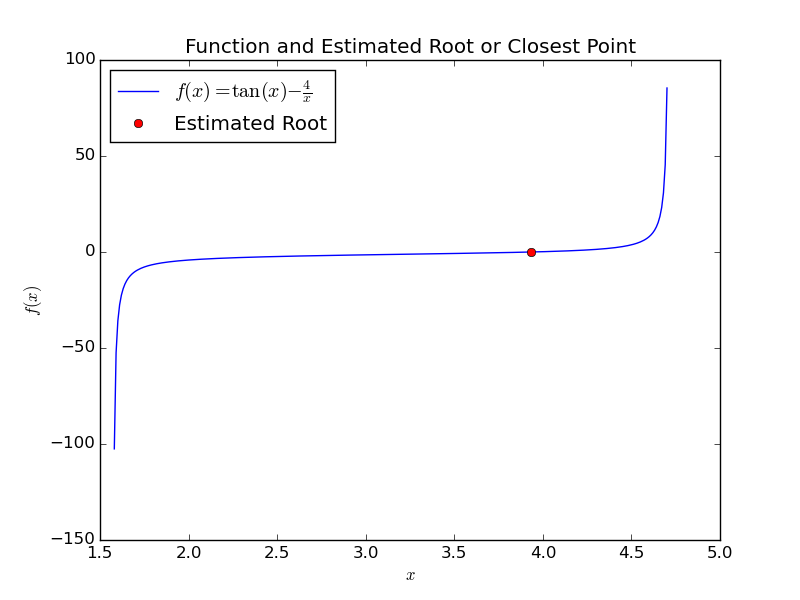
\includegraphics[width=.7\textwidth]{homework2_problem1_plot1}
  \caption{Interpolation and Extrapolation Results}
\end{figure}

We see here that the root is exceptionally close to what is expected.

\subsection{Data}

The results of the root finding, as well as finding the root using different ranges, are below:

\begin{verbatim}
Using Range: [ 1.58079632679 ,  4.70238898038 ]
Root at x = 3.93516165294
Using Range: [ 3.0 ,  4.5 ]
Root at x = 3.93516165294
Using Range: [ 2.5 ,  4.0 ]
Root at x = 3.93516165294
\end{verbatim}

\subsection{Analysis}

The algorithm will certainly find the root we desire, but may not do so very quickly. It may also get expectionally close to the root we desire, if it does not get there entirely.

\subsection{Interpretation}

The results are fairly reasonable, but a significant part of that has to do with the tolerance variable. In order to be sure we have found the root we desire and do not have any issues with roundoff erors, a tolerance value needs to be included so that we can stop the algorthm before machine precision stops the algorithm from working.

\subsection{Critique}

The tolerance value, as mentioned before, is fairly important for this function to work. It can be changed, but was used specfically because it gave good results. This brings in a lot of ambiguity, especially if the tolerance is set too high.

\pagebreak

\section{Problem 2}

\subsection{Problem Statement}

Write a program to solve $\tan(x) = a/x$ for $x$ in $(\pi/2, 3\pi/2)$, where $a = 5$, by using the secant method.
If necessary, you may combine the secant method with the bisection method. Compare your answer
with that of Problem 1. (10 pts).

\subsection{Method}

This program uses the secant method, as discussed in class, to try to find the root of the function in Problem 1. This is also fairly similar to the last problem, but since it requires three points in order to function, a third point is found by using bisection.

\subsection{Verification of Program}

Like the problem before, a plot has been used to verify the accuracy of the procedure.

\begin{figure}[h]
  \centering
    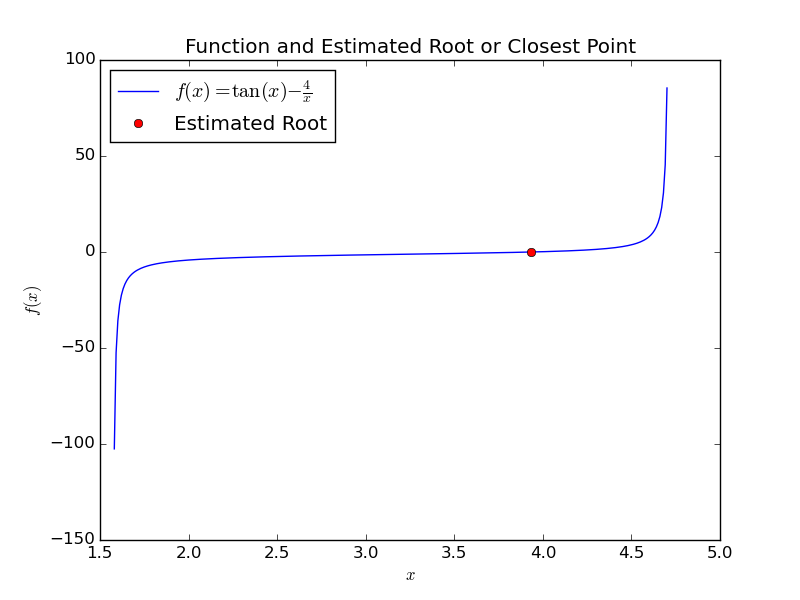
\includegraphics[width=.7\textwidth]{homework2_problem2_plot1}
  \caption{Interpolation and Extrapolation Results}
\end{figure}

As before, the plot looks reasonable and expected.

\subsection{Data}

The plot generated is included here.

The results of the root finding, as well as finding the root using different ranges, are below:

\begin{verbatim}
Found solution:  3.93516165294
Using Range: [ 1.58079632679 ,  4.70238898038 ]
Root at x = 3.93516165294
Using Range: [ 3.0 ,  4.5 ]
Root at x = 3.93516165294
Using Range: [ 2.5 ,  4.0 ]
Root at x = 3.93516165294
\end{verbatim}

\subsection{Analysis}

The root is found much faster, but has some issues when the bounds are too close to an asymptote. Since those conditions also make the function break, they have been omitted from the results.

\subsection{Interpretation}

The results, as with the last problem, are fairly stright forward and resonable.

\subsection{Critique}

The only real leap that needed to be made with this function was finding a good third point, and making a decision of which boundary to remove once the next point in the iteration has been found.

\pagebreak

\section{Problem 3}

\subsection{Problem Statement}

Write a program to solve the following linear algebraic equations using the Gauss Elimination method
with implicit partial pivoting. The implicit partial pivoting means: 
(i) First, all of the elements in
each row are normalized by the largest coefficient in the row. 
(ii) Second, rows are interchanged with
each other such that the diagonal elements become the largest (in magnitude) for each column. You
are supposed to do pivoting column by column. (20 pts)

\subsection{Method}

Gaussian Elimination has been implemented in this program, as discussed in class. In particular, the pivoting procedure has been done separately to the elimination so that the procedure without pivoting can be seen.

\subsection{Verification of Program}

The results have been compared to known results to verify that they were done correctly, along with a print of $A$ and $b$ in order to assure they were correct. See the "Data" section for the comparison.

\subsection{Data}

No plots were needed for these results. The results generated by the program are shown below:

\begin{verbatim}

Gauss, with pivoting:
A:
[[ 1.         -0.4         0.3         0.2       ]
 [ 0.          1.26666667  0.13333333 -0.46666667]
 [ 0.          0.          1.11842105 -0.28947368]
 [ 0.          0.          0.         -0.5       ]]
b:
[ 0.3        -0.2        -0.30263158  1.25      ]
x:
[ 0.68235294 -0.98235294 -0.91764706 -2.5       ]
Known Results: 
[ 0.68235294 -0.98235294 -0.91764706 -2.5       ]
Gauss, without pivoting:
A:
[[-0.5         0.5         1.         -0.5       ]
 [ 0.         -1.25       -1.25        0.25      ]
 [ 0.          0.          0.         -0.66666667]
 [ 0.          0.          0.                 inf]]
b:
[-0.5         1.75        1.66666667        -inf]
x:
[ nan  nan  nan  nan]
Known Results: 
[ 0.68235294 -0.98235294 -0.91764706 -2.5       ]
\end{verbatim}

\subsection{Analysis}

This function is fairly stable, as long as the pivorting is done before hand. As seen in the secondary results, the elimination without pivoting are unstable.

\subsection{Interpretation}

The results appear correct, and inparticular the no-pivoting results are unstable. It should be noted that while the results do return many warnings, there are no erros in the program that stop it from working.

\subsection{Critique}

The function actually has a few ways it could be written, and in particular it could use some checks to make sure that the matrices are usable. This is something that coud instead by done in the more advanced LU solvers discussed in later lectures.

\end{document}